\documentclass{standalone}

\usepackage{mathtools}
\usepackage{amsmath}
\usepackage{amssymb}
\usepackage{amsfonts}

%tikzpicture
\usepackage{tikz}
\usepackage{scalerel}
\usepackage{pict2e}
\usepackage{tkz-euclide}
\usetikzlibrary{calc}
\usetikzlibrary{patterns, arrows.meta}
\usetikzlibrary{shadows}
\usetikzlibrary{external}

%pgfplots
\usepackage{pgfplots}
\pgfplotsset{compat=newest}
\usepgfplotslibrary{statistics}
\usepgfplotslibrary{fillbetween}

%colors
\usepackage{xcolor}

\begin{document}

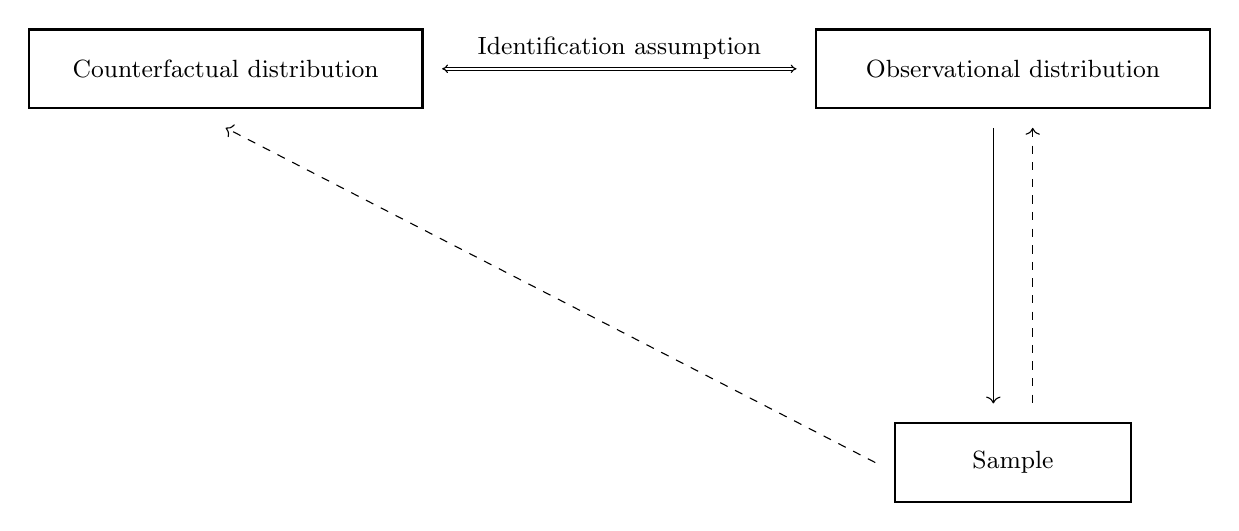
\begin{tikzpicture}

% Grid
\draw[white] (0, 0) grid (15, 6);

\draw[black, thick] (0, 5) rectangle (5, 6) node[pos=.5] {\small Counterfactual distribution} ;
\draw[black, thick] (10, 5) rectangle (15, 6) node[pos=.5] {\small Observational distribution} ;
\draw[{Implies}-{Implies},double] (5.25, 5.5) -- (9.75, 5.5) node[above, pos=.5] {\small Identification assumption} ;
\draw[black, thick] (11, 0) rectangle (14, 1) node[pos=.5] {\small Sample} ;
\draw[-To] (12.25, 4.75) -- (12.25, 1.25) ;
\draw[dashed, To-] (12.75, 4.75) -- (12.75, 1.25) ;
\draw[dashed, -To] (10.75, 0.5) -- (2.5, 4.75) ;


\end{tikzpicture}


\end{document}
